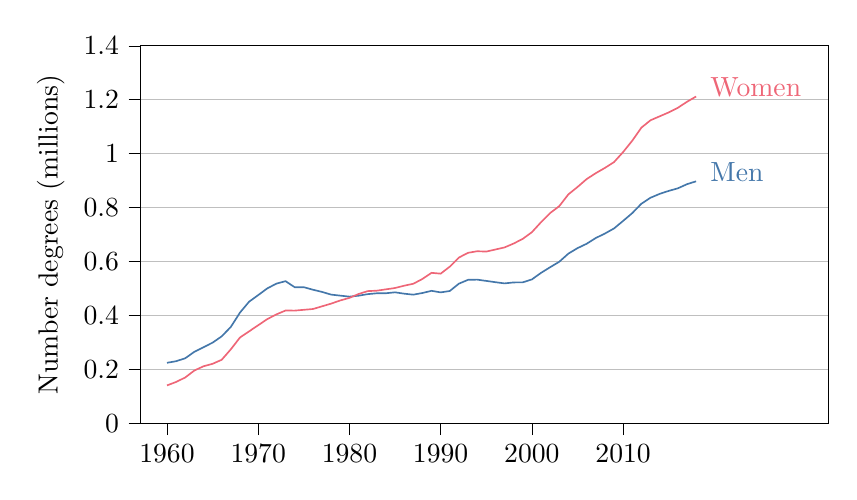
\begin{tikzpicture}
% This file was created by tikzplotlib v0.9.2.
\definecolor{color0}{rgb}{0.266666666666667,0.466666666666667,0.666666666666667}
\definecolor{color1}{rgb}{0.933333333333333,0.4,0.466666666666667}

\begin{axis}[
height=6.376357092455836cm,
tick align=outside,
tick pos=left,
width=10.317162499999998cm,
x grid style={white!69.0196078431373!black},
xmin=1957.1, xmax=2032.5,
xtick style={color=black},
xtick={1960,1970,1980,1990,2000,2010},
xticklabels={\(\displaystyle 1960\),\(\displaystyle 1970\),\(\displaystyle 1980\),\(\displaystyle 1990\),\(\displaystyle 2000\),\(\displaystyle 2010\)},
ylabel={Number degrees (millions)},
ymajorgrids,
ymin=0, ymax=1.4,
ytick style={color=black},
ytick={0,0.2,0.4,0.6,0.8,1,1.2,1.4},
yticklabels={\(\displaystyle 0\),\(\displaystyle 0.2\),\(\displaystyle 0.4\),\(\displaystyle 0.6\),\(\displaystyle 0.8\),\(\displaystyle 1\),\(\displaystyle 1.2\),\(\displaystyle 1.4\)}
]
\addplot [semithick, color0]
table {%
1960 0.224537968635559
1961 0.230455994606018
1962 0.2413090467453
1963 0.26534903049469
1965 0.299286961555481
1966 0.322710990905762
1967 0.3576819896698
1968 0.410594940185547
1969 0.451097011566162
1970 0.475594043731689
1971 0.500590085983276
1972 0.518190979957581
1973 0.527312994003296
1974 0.504841089248657
1975 0.504925012588501
1976 0.495545029640198
1977 0.487347006797791
1978 0.477344036102295
1980 0.469882965087891
1981 0.473363995552063
1982 0.479140043258667
1983 0.482318997383118
1984 0.4825279712677
1985 0.485923051834106
1986 0.480854034423828
1987 0.477203011512756
1988 0.483345985412598
1989 0.491487979888916
1990 0.48564600944519
1991 0.490826010704041
1992 0.517989993095398
1993 0.532243013381958
1994 0.532928943634033
1996 0.523488998413086
1997 0.518990993499756
1998 0.522558927536011
1999 0.522891998291016
2000 0.533735036849976
2001 0.557978987693787
2002 0.579033017158508
2003 0.599171996116638
2004 0.629392027854919
2005 0.649704933166504
2006 0.66592800617218
2007 0.687217950820923
2008 0.703808069229126
2009 0.722702980041504
2010 0.750731945037842
2011 0.779560089111328
2012 0.814333915710449
2013 0.836575031280518
2014 0.850880980491638
2015 0.862040996551514
2016 0.871549010276794
2017 0.886856079101562
2018 0.897544026374817
};
\addplot [semithick, color1]
table {%
1960 0.140635967254639
1961 0.153504967689514
1962 0.170110940933228
1963 0.195917010307312
1964 0.211583971977234
1965 0.220828056335449
1966 0.235823035240173
1967 0.274606943130493
1968 0.318249940872192
1971 0.386682987213135
1972 0.404170989990234
1973 0.418462991714478
1974 0.418092012405396
1976 0.424003958702087
1978 0.444046020507812
1979 0.455806016921997
1980 0.465256929397583
1981 0.479634046554565
1982 0.490370035171509
1983 0.491989970207214
1985 0.50189995765686
1986 0.510484933853149
1987 0.517626047134399
1988 0.535408973693848
1989 0.558169007301331
1990 0.555091023445129
1991 0.581097006797791
1992 0.614879012107849
1993 0.632375001907349
1994 0.638270020484924
1995 0.636955976486206
1997 0.652374982833862
1998 0.666815042495728
1999 0.684229016304016
2000 0.708883047103882
2001 0.745826005935669
2002 0.779849052429199
2003 0.805441975593567
2004 0.849164962768555
2005 0.87644100189209
2006 0.905745983123779
2007 0.927672982215881
2008 0.947183012962341
2009 0.968661069869995
2010 1.00603902339935
2011 1.04807901382446
2012 1.09642803668976
2013 1.12388396263123
2015 1.15306401252747
2016 1.17018795013428
2017 1.19238698482513
2018 1.2120840549469
};
\draw (axis cs:2018.5,0.897544) node[
  anchor=base west,
  text=color0,
  rotate=0.0
]{Men};
\draw (axis cs:2018.5,1.212084) node[
  anchor=base west,
  text=color1,
  rotate=0.0
]{Women};
\end{axis}



\end{tikzpicture}
\caption{Number of Bachelor's Degrees awarded in US 4-year colleges. Source: IPEDS; Snyder (2013).}
